\setcounter{section}{18}

\section{Частично упорядоченные множества. Диаграмма Хассе. Изоморфизм. Описание попарно неизоморфных ч.у.м. для 3-х и 4-х элементов. Минимальные, максимальные, наибольшие и наименьшие элементы.}

Множество A с заданным на нем частичным порядком R называется \textbf{частично упорядоченным множеством (ЧУМ)} и обозначается (A; R). \textbf{Отношением (нестрогого частичного) порядка} называется любое рефлексивное, антисимметричное и транзитивное отношение. \\ \par

\textbf{Диаграммой Хассе} называется ориентированный граф без циклов, по которому отношение порядка строится так: $a \leqslant b$, если из a в b идёт ориентированный путь. Диаграмму Хассе для отношения можно получить из ориентированного графа, его изображающего, выкидыванием петель и таких рёбер между вершинами a и c, если есть вершина b, такая, что: $a < b < c$. Кроме того, вместо рисования стрелок граф располагают так, чтобы большие элементы находились выше. \par
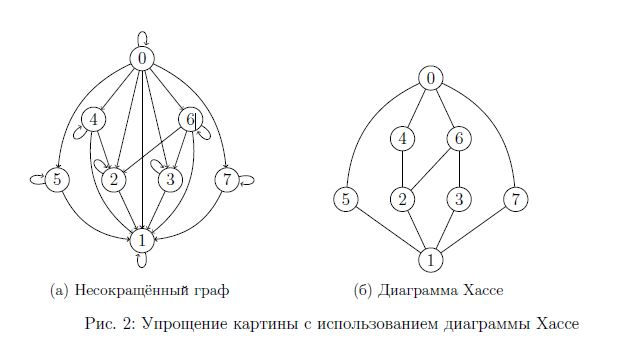
\includegraphics{images/19_hasse} \par

\textbf{Изоморфизмом} упорядоченных множеств $(A, \leqslant_A)$ и $(B, \leqslant_B)$ называется биекция $f: A \rightarrow B$, для которого выполнено свойство:  $x \leqslant_A y \Leftrightarrow f(x) \leqslant_B f(y)$. Обозначение: $A \simeq B$. \\ \par
\emph{Описание попарно неизоморфных ч.у.м. для 3-х и 4-х элементов.} Доказательство основывается на попарно неизоморфных графах без петель и кратных рёбер (для n=3 их 4, для n=4 их 11) \par
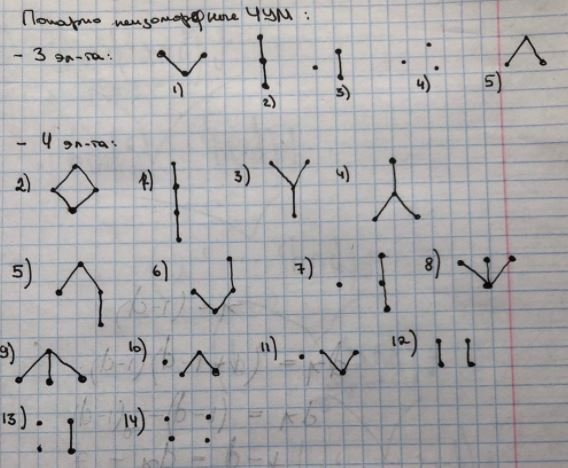
\includegraphics{images/19_pos} \\ \par

Элемент $x \in A$ \textbf{наибольший} в упорядоченном множестве $(A, \leqslant_A)$, если $\forall y \in A: y \leqslant_A x$. Элемент $x \in A$ \textbf{максимальный} в упорядоченном множестве $(A, \leqslant_A)$, если $\nexists y \in A : x <_A y$. Наименьший и минимальный элементы определяются аналогично. \\ \par

\emph{Свойства максимальных/наибольших/минимальных/наименьших элементов:} \\
1. Наибольший элемент всегда является максимальным, причём единственным; \\
2. Максимальных элементов может быть несколько; \\
3. Единственный максимальный элемент не всегда является наибольшим. \\ \par
$\blacktriangle$
1. Если x наибольший, то $x \leqslant y$ для всех $y \in A$. Поэтому $x \nless y$ для всех y. Поэтому он максимален. Любой другой элемент будет меньше наибольшего
и потому не будет максимальным. \par
2. Например, можно взять натуральные числа от 1 до 10 и отношение делимости.
Максимальными будут числа 6, 7, 8, 9, 10: на них никакое число из этого интервала
не делится. \par
3. Например, можно взять множество $\{ 3 \} \cup \{2^n | n \in \mathbb{N}\}$ с отношением делимости. 3 является единственным максимальным элементом, т.к. на любое другое делится ещё какое-то число. Но наибольшего элемента тут нет.
$\blacksquare$